\begin{tikzpicture}[align=center, font={\footnotesize}]

    \matrix[inner sep=0pt, column sep=3em, row sep=1em, ampersand replacement=\nextcell] (mtx) {

        \node[inner sep=0pt] (r1) {State change vs. no state change.\\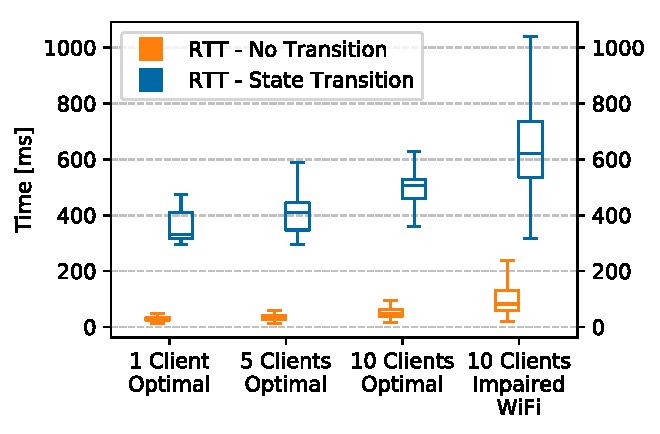
\includegraphics[width=.42\linewidth]{plots/rtt_fb_vs_nofb.pdf}};
        \nextcell \node[inner sep=0pt] (r2) {Times by pipeline segments.\\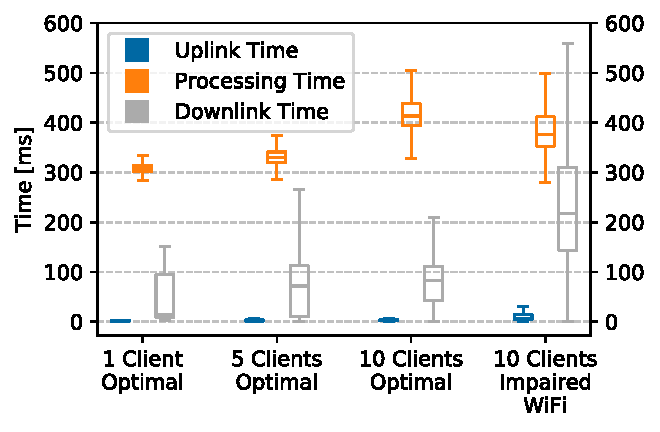
\includegraphics[width=.42\linewidth]{plots/box_feedback.pdf}}; \\

        \node[inner sep=0pt] (r3) {RTT by task step.\\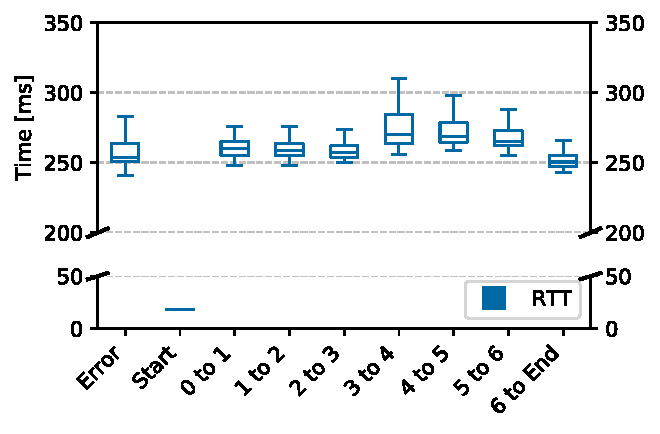
\includegraphics[width=.42\linewidth]{plots/box_taskstep.pdf}};
        \nextcell \node[inner sep=0pt] (r4) {%
        Reference latency bounds for LEGO\\(\textcite{Chen:AnEmpiricalStudyOfLatency})\\
        \ \\
        \begin{tabular}{@{}ll@{}}
            \toprule
            Latency {[}ms{]} & Quality   \\ \midrule
            $< 600$          & Excellent \\
            $600-2700$       & Impaired  \\
            $> 2700$         & Unusable  \\ \bottomrule
        \end{tabular}%
    }; \\
    };

\end{tikzpicture}